% Gerado de produtos auditados por relatorio_tp2.py.
\section{Resultados da Otimização Multiobjetivo}
\label{sec:resultados_tp2}
A coleta reuniu 160 buscas, com 5 varreduras por abordagem. Todas as buscas, inclusive as que não encontraram viável, permanecem contabilizadas. A auditoria recalculou objetivos e restrições das composições, verificou proveniência e recompôs os arquivos em 3D.
\begin{table}[H]\centering\small
\caption{Contabilidade das buscas e uniões não dominadas por método.}
\label{tab:tp2_metodos}
\begin{tabular}{lrrrrr}\toprule
Método & Runs & Viáveis & Sem viável & Composições ND & Vetores ND \\ \midrule
Soma ponderada & 80 & 80 & 0 & 3961 & 3830 \\
$\varepsilon$-restrito & 80 & 45 & 35 & 1206 & 1182 \\
\bottomrule\end{tabular}\end{table}
% Gerado por figuras_tp2.py; não editar números manualmente.
\begin{table}[H]\centering
\caption{Resultados por varredura. ND: composições não dominadas em três objetivos.}
\label{tab:tp2_repeticoes}
\begin{tabular}{llrrrr}\toprule
Método & Semente-base & Runs & Viáveis & Sem viável & ND \\ \midrule
Ponderada & 42 & 16 & 16 & 0 & 1617 \\
Ponderada & 123 & 16 & 16 & 0 & 1963 \\
Ponderada & 456 & 16 & 16 & 0 & 1861 \\
Ponderada & 789 & 16 & 16 & 0 & 1744 \\
Ponderada & 1011 & 16 & 16 & 0 & 1954 \\
$\varepsilon$-restrito & 42 & 16 & 9 & 7 & 657 \\
$\varepsilon$-restrito & 123 & 16 & 9 & 7 & 790 \\
$\varepsilon$-restrito & 456 & 16 & 9 & 7 & 674 \\
$\varepsilon$-restrito & 789 & 16 & 9 & 7 & 634 \\
$\varepsilon$-restrito & 1011 & 16 & 9 & 7 & 741 \\
\bottomrule\end{tabular}
\end{table}

\begin{table}[H]\centering\small
\caption{Intervalos dos três objetivos nas uniões ND. Extremos de objetivos diferentes podem pertencer a composições diferentes.}
\label{tab:tp2_intervalos}
\resizebox{\linewidth}{!}{\begin{tabular}{lrrr}\toprule
Método & Custo (milhões de R\$) & Desvio $SiO_2$ (p.p.$^2$) & Desvio $Al_2O_3$ (p.p.$^2$) \\ \midrule
Soma ponderada & \num{60.740} -- \num{65.680} & \num{2.407} -- \num{6.872} & \num{1.452} -- \num{5.442} \\
$\varepsilon$-restrito & \num{60.460} -- \num{64.520} & \num{3.039} -- \num{6.616} & \num{2.325} -- \num{5.822} \\
\bottomrule\end{tabular}}\end{table}
\begin{table}[H]\centering\small
\caption{Exemplos de composições efetivamente encontradas nos extremos marginais de cada método. Cada linha é uma alternativa completa, não uma combinação de mínimos.}
\label{tab:tp2_extremos}
\begin{tabular}{llrrr}\toprule
Método & Extremo & Custo (milhões R\$) & $f_2$ (p.p.$^2$) & $f_3$ (p.p.$^2$) \\ \midrule
Soma ponderada & $f_1$ mínimo & \num{60.740} & \num{6.625} & \num{4.959} \\
Soma ponderada & $f_2$ mínimo & \num{63.700} & \num{2.407} & \num{3.284} \\
Soma ponderada & $f_3$ mínimo & \num{65.660} & \num{5.498} & \num{1.452} \\
$\varepsilon$-restrito & $f_1$ mínimo & \num{60.460} & \num{6.343} & \num{5.706} \\
$\varepsilon$-restrito & $f_2$ mínimo & \num{63.120} & \num{3.039} & \num{3.640} \\
$\varepsilon$-restrito & $f_3$ mínimo & \num{64.460} & \num{3.783} & \num{2.325} \\
\bottomrule\end{tabular}\end{table}
\begin{table}[H]\centering\small
\caption{Esforço efetivo. Tempos de busca são decorridos, não de CPU, e excluem persistência, consolidação e auditoria.}
\label{tab:tp2_esforco}
\begin{tabular}{lrrr}\toprule
Método & Avaliações & Tempo de busca (s) & Média por run (s) \\ \midrule
Soma ponderada & \num{800000} & \num{955.32} & \num{11.94} \\
$\varepsilon$-restrito & \num{800000} & \num{881.86} & \num{11.02} \\
\bottomrule\end{tabular}\end{table}
A coleta completa, incluindo persistência e consolidação, levou \num{46.01} minutos. A auditoria e geração de figuras consumiram \num{13.29} minutos adicionais. Esses valores não se confundem com a soma dos tempos dos solvers.
\subsection{Projeções e variabilidade entre varreduras}
As figuras mantêm os arquivos ND de cada repetição antes da projeção. Um ponto aparentemente dominado em 2D pode permanecer não dominado em 3D. A mesma composição pode aparecer nas cinco varreduras, com todas as origens preservadas.
\begin{figure}[H]\centering
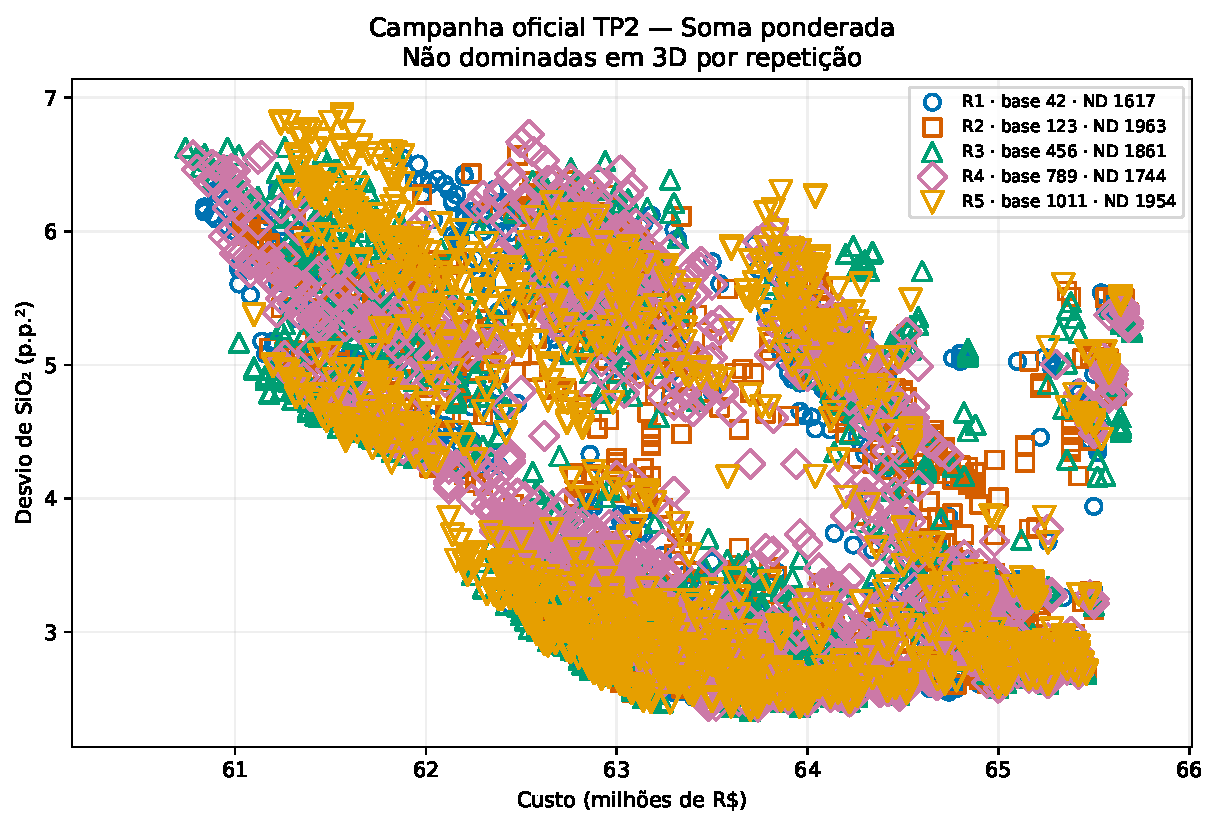
\includegraphics[width=0.88\linewidth]{results/tp2/figuras/ponderada_f1_f2.pdf}
\caption{Soma ponderada: projeção $f_1\times f_2$, com as repetições identificadas.}
\label{fig:tp2_ponderada_1_2}
\end{figure}
\begin{figure}[H]\centering
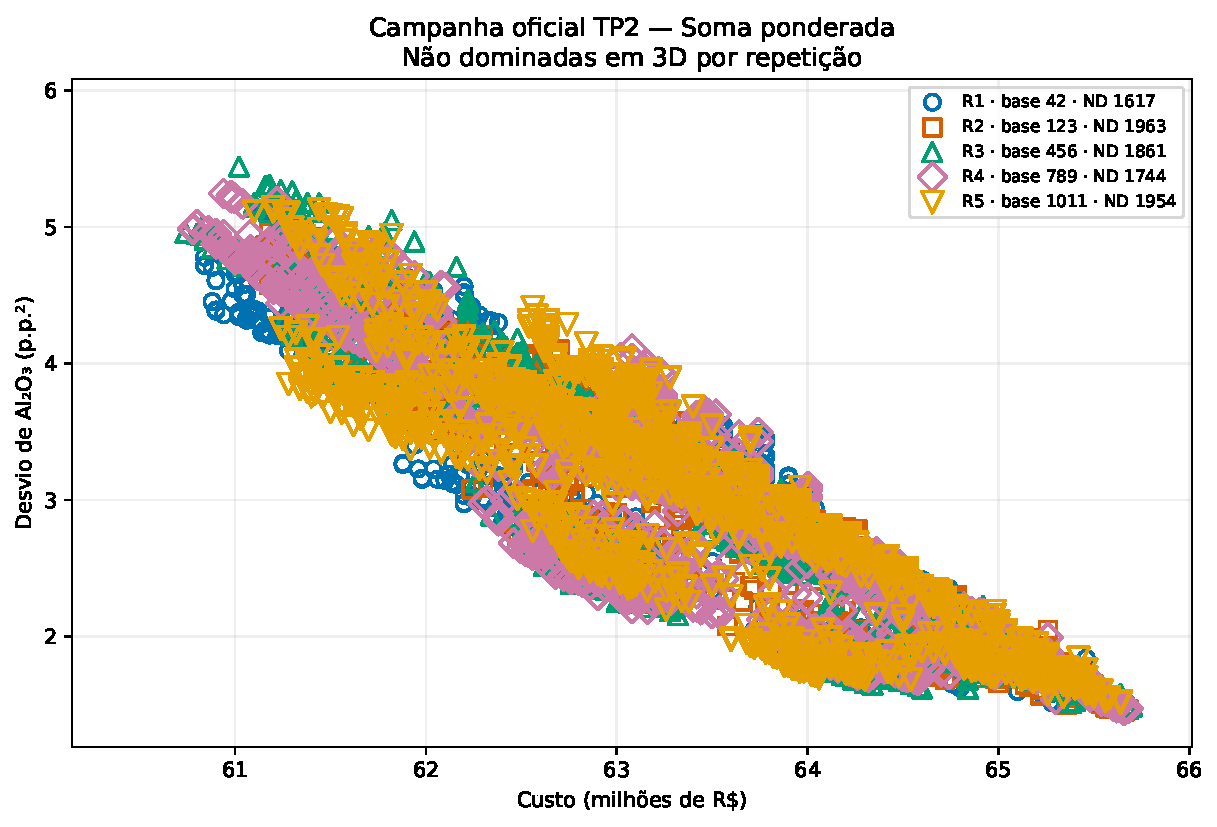
\includegraphics[width=0.88\linewidth]{results/tp2/figuras/ponderada_f1_f3.pdf}
\caption{Soma ponderada: projeção $f_1\times f_3$, com as repetições identificadas.}
\label{fig:tp2_ponderada_1_3}
\end{figure}
\begin{figure}[H]\centering
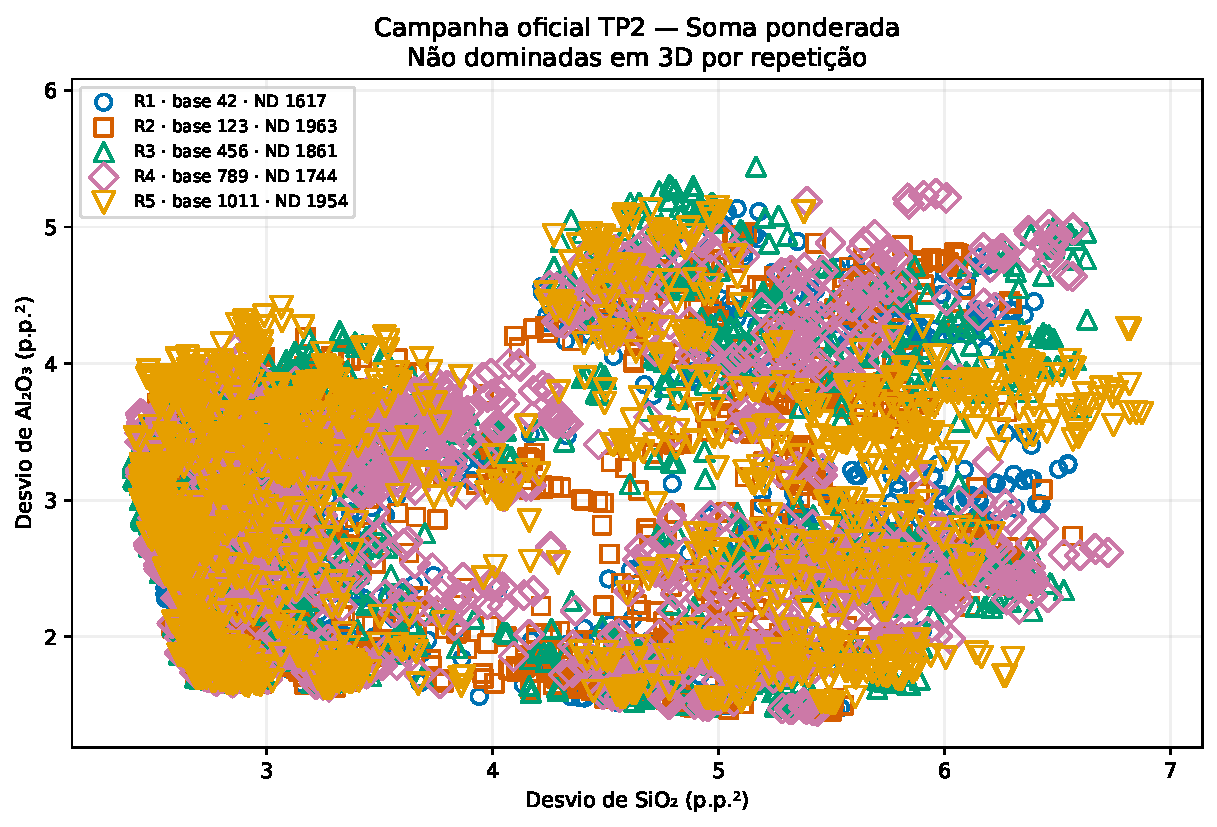
\includegraphics[width=0.88\linewidth]{results/tp2/figuras/ponderada_f2_f3.pdf}
\caption{Soma ponderada: projeção $f_2\times f_3$, com as repetições identificadas.}
\label{fig:tp2_ponderada_2_3}
\end{figure}
\begin{figure}[H]\centering
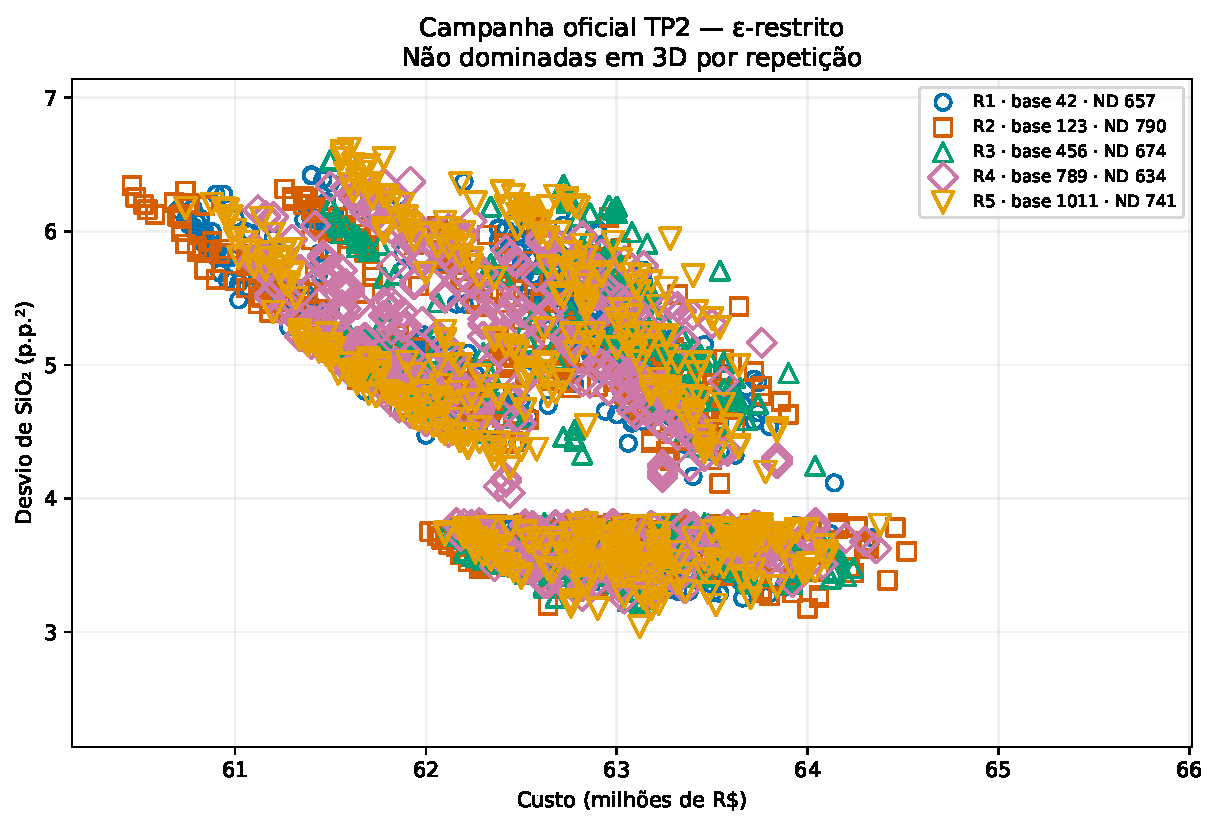
\includegraphics[width=0.88\linewidth]{results/tp2/figuras/epsilon_f1_f2.pdf}
\caption{$\varepsilon$-restrito: projeção $f_1\times f_2$, com as repetições identificadas.}
\label{fig:tp2_epsilon_1_2}
\end{figure}
\begin{figure}[H]\centering
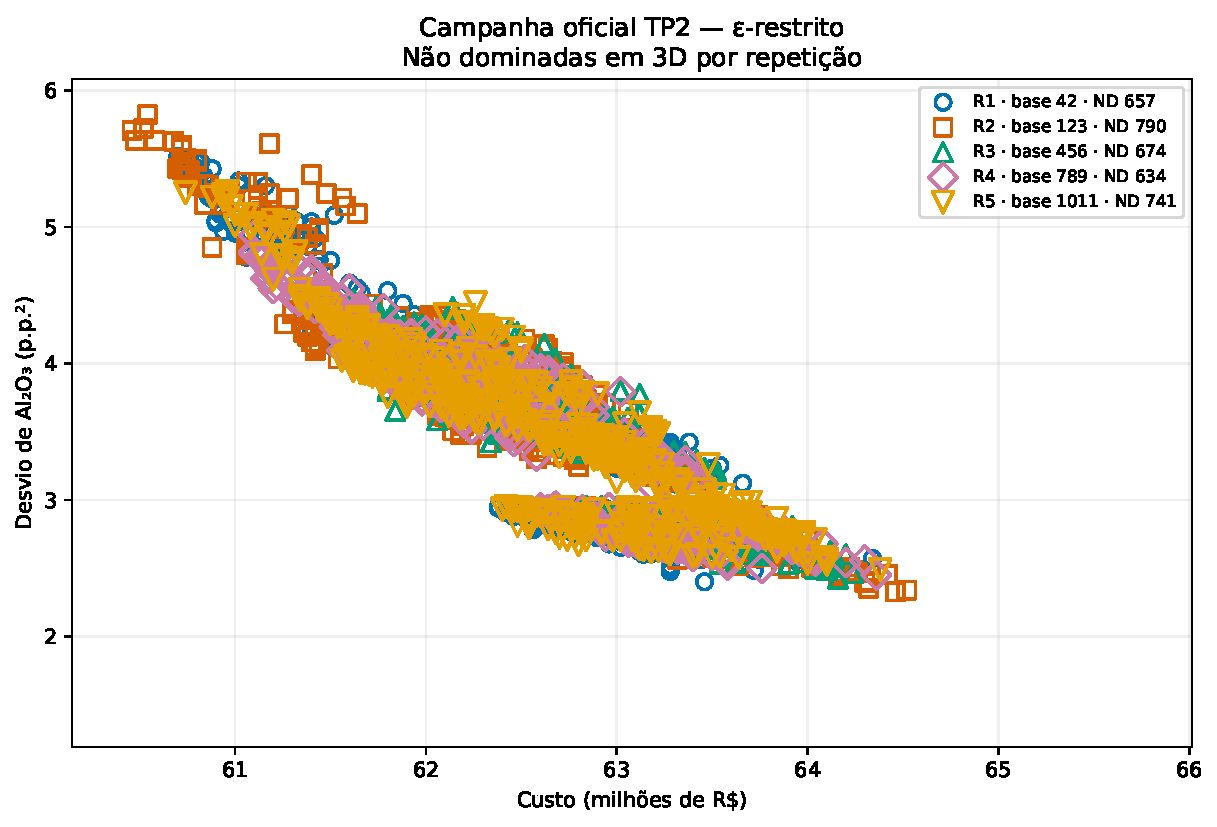
\includegraphics[width=0.88\linewidth]{results/tp2/figuras/epsilon_f1_f3.pdf}
\caption{$\varepsilon$-restrito: projeção $f_1\times f_3$, com as repetições identificadas.}
\label{fig:tp2_epsilon_1_3}
\end{figure}
\begin{figure}[H]\centering
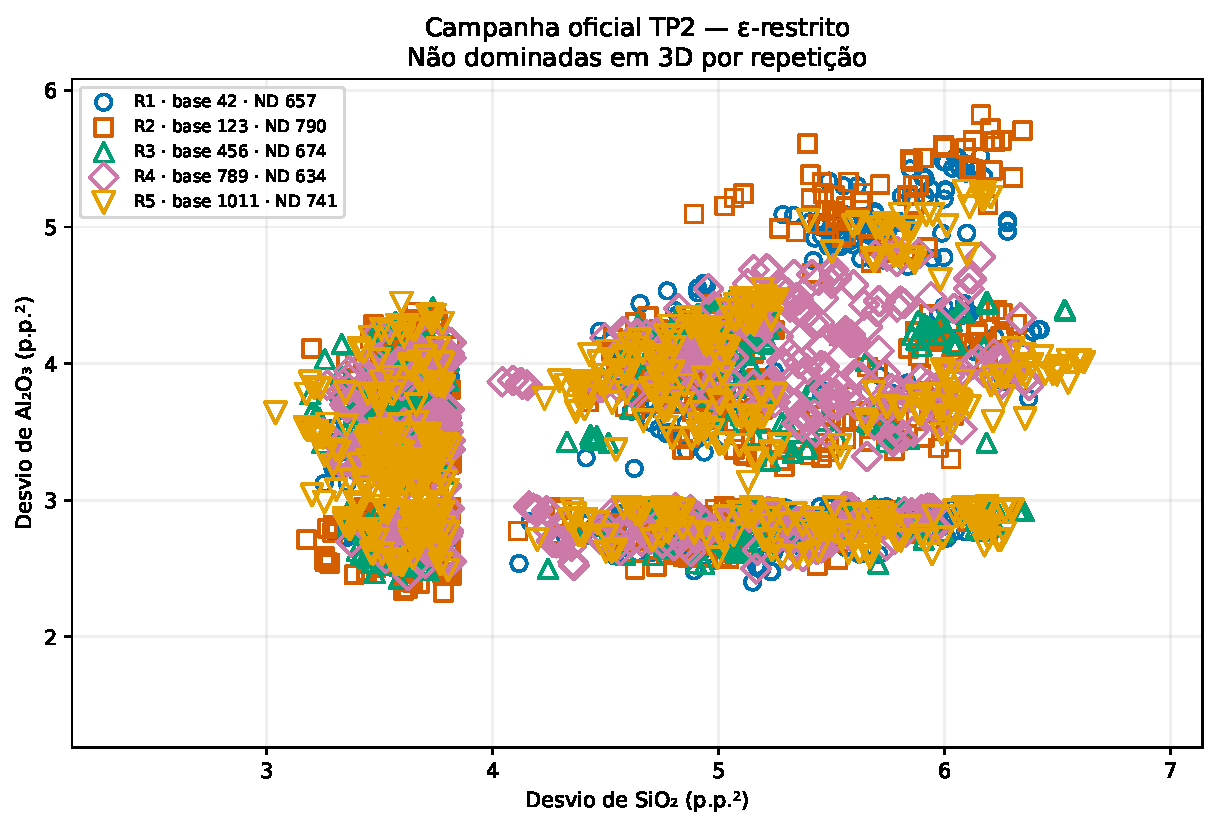
\includegraphics[width=0.88\linewidth]{results/tp2/figuras/epsilon_f2_f3.pdf}
\caption{$\varepsilon$-restrito: projeção $f_2\times f_3$, com as repetições identificadas.}
\label{fig:tp2_epsilon_2_3}
\end{figure}
\subsection{Comparação descritiva das aproximações}
Entre os vetores distintos encontrados, a união ponderada domina estritamente \num{66.24}\% dos vetores da união $\varepsilon$-restrita; no sentido inverso, a fração é \num{3.26}\%. Essa comparação usa três objetivos e apenas as amostras encontradas; não certifica superioridade global dos métodos.
Há 0 vetores de objetivos iguais e 0 composições físicas comuns entre as uniões. Essas contagens são distintas da quantidade de pontos sobrepostos em uma projeção.
O escalar principal não é comparável entre métodos ou configurações. A comparação deve considerar os três objetivos brutos, as mesmas referências, o teto comum e o esforço efetivamente realizado. Mais composições no arquivo não provam melhor método. As cinco varreduras, e não as buscas individuais, representam as repetições do desenho.
